\section*{21. AdaBoost}
\subsection*{Boosting Methods}
\begin{itemize}
    \item
        Learning technique, that combines output of many weak classifiers to produce a powerful committee
    \item
        Weak classifier: error rate which is only slightly better than random guessing
    \item
        Idea: Sequentially apply the weak classifier to repeatedly modified versions of the data\\
    \item
        Consider a two-class problem with $y \in \{-1, +1\}$
    \item
        Given a set of observations $D = \{(x_i, y_i), i=1, \dots, N\}$ and a classifier $G(x)$, the error rate on the training sample is:
        $$err = \ffrac{1}{N} \sum_{i=1}^{N} I(y_i \neq G(x_i))$$
        where I is the indicator function 
    \item
        Sequentially applied weak classiefers produce a sequence $G_m(x)$ with $m = 1,2,\dots,M$
    \item
        The combined preditction is then:
        $$G(x) = sign(\sum_{m=1}^{M} \alpha_m G_m(x))$$
    \item
        The weighting factors $\alpha_1, \dots, \alpha_M$ are computed by the boosting algorithm
        \begin{figure}[H]
            \centering
            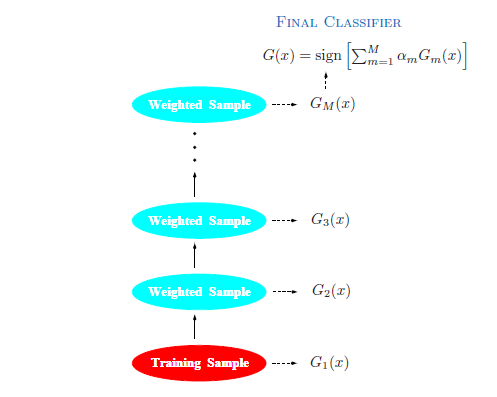
\includegraphics[scale=1]{figures/ada}
        \end{figure}
    \item
        Modification on the data:
        \begin{itemize}
            \item
                Each boosting step consists of applying weights $w_1, w_2, \dots, w_N$ to the training samples
            \item
                Initially, the weights are set to $w_i = 1/N \rightarrow$ first classifier is trained the usual way
            \item
                At step $m$ the misclassified observations from $G_{m-1}$ have increased weights
            \item
                The weights for correctly classified samples from $G_{m-1}$ have decreased weights
            \item
                Effect: Each successive classifier is forced to concentrate more on those observations that were misclassified by the previous ones
        \end{itemize}
    \item
        AdaBoost algorithm:
\begin{lstlisting}[mathescape]
    Initialize weights: $w_i = 1/N, i = 1, \dots, N$
    $m = 1$
        Fit classifier $G_m(x)$ to training data using $w$
        Compute classification error: $err_m = \ffrac{\sum_{i=1}^N w_i I(y_i \neq G_m(x_i))}{\sum_{i=1}^N w_i}$
        Compute classifier weights: $\alpha_m = log(\ffrac{1-err_m}{err_m})$
        Compute new sample weights:
        $w_i = w_i \; e^{\alpha_m I(y_i \neq G_m(x_i))}, i=1,\dots,N$
        $m = m+1$
    $m = M$
    Output: $G(x) = sign(\sum_{m=1}^M \alpha_m G_m(x))$
\end{lstlisting}
    \item
        Discrete AdaBoost, because $G_m(x)$ returns a discrete class label. Can be modified to return real-valued prediction in the interval $[-1, 1]$
\end{itemize}
\subsection*{Exponential Loss}
\begin{itemize}
    \item
        Boosting fits and additive model in a set of elementary basis functions:
        $$ f_M(x) = \sum_{m=1}^M \beta_m b(x; \gamma_m)$$
        where $\beta_m$ are expansion coefficients and $b(x; \gamma_m)$ is a basis function given a set of parameters $\gamma_m$
    \item
        Expansion models are typically fit by minimizing a loss function $L$ averaged over the training data:
        $$ \underset{\{\beta_m, \gamma_m\}_1^M}{min} \{\sum_{i=1}^{N} L(y_i, f_M(x_i))\}$$
    \item
        Forward stagewise modeling approximates the solution:
\begin{lstlisting}[mathescape]
    Initialize $f_0(x) = 0$
    For $m=1$ to M:
        Compute
            $(\beta_m, \gamma_m) = \underset{\beta, \gamma}{argmin} \sum_{i=1}^N L(y_i, f_{m-1}(x_i) + \beta b(x_i;\gamma))$
        Set $f_m(x) = f_{m-1}(x) + \beta_m b(x;\gamma_m)$
\end{lstlisting}
    \item
        AdaBoost is equivalent to a forward stagewise additive modeling using an exponential loss function:
        $$L(y, f(x)) = exp(-y f(x))$$
    \item
        Proof: See lecture slides
        \begin{figure}[H]
            \centering
            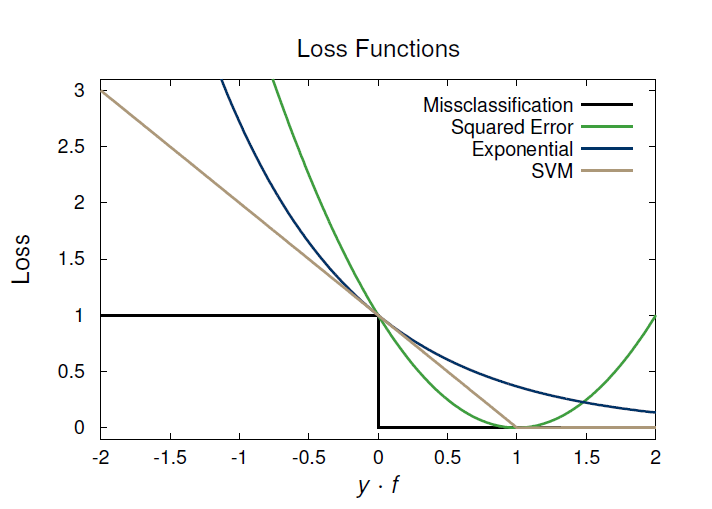
\includegraphics[scale=0.7]{figures/loss_funcs}
        \end{figure}
    \item
        AdaBoost criterion yields a monotone decreasing function of the margin $yf(x)$
    \item
        The goal of the classification algorithm is to produce positive margins as frequently as possible
    \item
        Thus, any loss criterion should penalize negative margins more heavily than positive ones
    \item
        Exponential criterion concentrates much more influence on observations with large negative margins $\rightarrow$ Noisy data and wrong class labels make AdaBoost performance degrade rapidly
\end{itemize}
\subsection*{Viola and Jones}
\subsubsection*{Features}
\begin{itemize}
    \item
        Look at sub-window $(24 \times 24)$ of original image
    \item
        Four basic features adapted from Haar basic function:
        \begin{figure}[H]
            \centering
            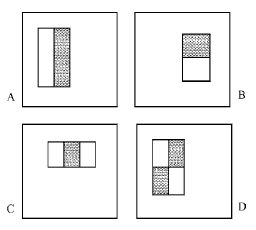
\includegraphics[scale=0.7]{figures/viola1}
        \end{figure}
    \item
        Calculated by subtracting the sum of pixels in the white are from the sum of the pixels in the gray area
    \item
        Yields $> 160000$ features for every sub-window (depending on scale, position and type of used basic feature)
    \item
        Efficient computation via Integral Image $II(x, y) = \sum_{x'\leq x, y' \leq y} I(x',y')$
\end{itemize}
\subsubsection*{Boosting}
\begin{itemize}
    \item
        Smaller number of features seems sufficient
    \item
        Boosting can be seen as as having a large set of classification functions, choosing the best function at every stage and giving the good ones a big weight
    \item
        Idea: Restrict classification functions to each depend on a single feature only
    \item
        A weak classifier $G_j(x)$ consists of a feature $x_j$, and optimal threshold $\theta_j$, and a parity $s_j$ to indicate the direction of the inequality
        $$G_j(x) = 1 \text{ if } s_j f_j(x) < s_j \theta_j \text{ else } 0$$
        with $x$ being a sub-window of an image
    \item
        AdaBoost can be interpreted as an effective feature selection algorithm, where the single rectangle feature is selected which best seperates the observation and for each feature, an optimal threshold is determined
    \item
        First and second feature selected by AdaBoost:

        \begin{figure}[H]
            \centering
            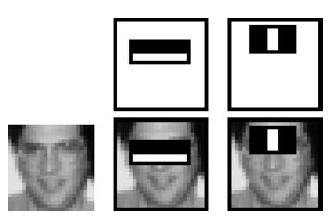
\includegraphics[scale=0.7]{figures/viola2}
        \end{figure}
\end{itemize}
\subsubsection*{Classifier Cascade}
\begin{itemize}
    \item
        Despite the efficiency of the feature computation, evalutating the full AdaBoost sequence on all sub-windows of the image takes too much time
    \item
        Idea of cascaded classifiers:
        \begin{itemize}
            \item
                Simpler classifiers used to reject the majority of sub-windows
            \item
                Each stage again created by AdaBoost
            \item
                Stage 1 uses the two features shown before; detects 100\% faces with FPR of around $40$\%
            \item
                Goal is to reject as many negatives as possible at the earliest stage of the processing
        \end{itemize}
        \begin{figure}[H]
            \centering
            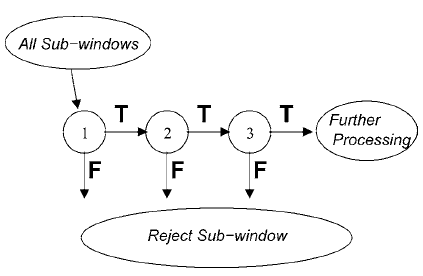
\includegraphics[scale=0.8]{figures/viola3}
        \end{figure}
    \item
        Training of the cascade:
        \begin{itemize}
            \item
                Subsequent classifiers are trained using only those examples which pass through all the previous stages
            \item
                The next classifier faces a more difficult task than the previous one
            \item
                Trade-off between more features achieving higher detection rates and lower FPRs while requiring more computation time
        \end{itemize}
    \item
        Final classifier has 32 layer cascade
    \item
        Number of stages and features adapted until false postivie rate on validation was nearly zero while maintaining high correct rate
\end{itemize}
